\providecommand{\tituloDocumento}{Guía}
\providecommand{\subtituloDocumento}{El triángulo y sus propiedades}

\documentclass{sn-guia}

\begin{document}
%
\raggedright
\begin{tcbraster}[enhanced,raster columns=2,raster width=\linewidth,raster column skip=3pt,raster force size=false]
    \begin{caja}[title={\sffamily\scshape\bfseries Nombre},height=30pt,add to width=4cm]
    \end{caja}
    \begin{caja}[title={\sffamily\scshape\bfseries Curso},height=30pt,add to width=-4cm]
    \end{caja}    
    \begin{caja}[title={\sffamily\scshape\bfseries Fecha},height=30pt]
    \end{caja}                
    \begin{caja}[title={\sffamily\scshape\bfseries Profesor},height=30pt]
    \end{caja}
\end{tcbraster}

%\vspace{5mm}
%\begin{tcolorbox}[boxrule=1pt,colback=white,leftrule=3mm]
%    {\bfseries Objetivo:} Resuelva el problema que se encuentra a continuación. Para esto, no olvide 
%    incluir un desarrollo pertinente y la respuesta al enunciado en los espacios señalizados.        
%\end{tcolorbox}

%\parte 
\begin{tcolorbox}[boxrule=1pt,colback=white,leftrule=3mm,grow to left by=-1cm,
    grow to right by=-1cm, enlarge top by=5mm, enlarge bottom by=5mm]
    {\bfseries\sffamily\large Competencias a desarrollar:}
    \begin{itemize}\raggedright
        \item Construye e interpreta modelos geométricos de ángulos y triángulos al resolver problemas derivados de situaciones reales, hipotéticas o teóricas.
        \item Cuantifica y representa magnitudes angulares y de longitud en ángulos y triángulos identificados en situaciones reales, hipotéticas o teóricas.
        \item Interpreta diagramas y textos con símbolos propios de ángulos y triángulos.
    \end{itemize}
\end{tcolorbox}

\begin{multicols}{2}
    [\section*{Principio de Euclides}]
    Uno de los principios fundamentales de la geometría, dice que si $l_1$ y $l_2$ son rectas se cumple que:
    \begin{itemize}[]
        \item $\alpha + \beta = 180^{\circ}$
        \item $\gamma + \delta = 180^{\circ}$
    \end{itemize}
    Si además de lo anterior, se cumple que $l_1 \parallel l_2$, entonces:
    \begin{itemize}[]
        \item $\alpha = \gamma$
        \item $\beta = \delta$
    \end{itemize}

    \begin{center}
        \begin{tikzpicture}[rotate=30]
            \draw[<->,name path=A-B,line width=1pt] (0,0) coordinate (A) -- ++(5,0) coordinate (B) node[right] {$l_2$};
            \draw[<->,name path=C-D,line width=1pt] (A) ++(0,2) coordinate (C) -- ++(5,0) coordinate (D) node[right] {$l_1$};
            \draw[<->,name path=E-F,line width=1pt] ($(A)!0.3!(B)!1.5cm!250:(B)$) coordinate (E) -- ($(C)!0.7!(D)!1.5cm!70:(D)$) coordinate (F);
            \draw[name intersections={of=C-D and E-F,by=vCD}] pic ["$\alpha$",draw,<->,angle eccentricity=1.2,angle radius=1cm] {angle = D--vCD--F};
            \draw pic ["$\beta$",draw,<->,angle eccentricity=1.2,angle radius=0.8cm] {angle = F--vCD--C};
            \draw pic ["$\alpha$",draw,<->,angle eccentricity=1.2,angle radius=1cm] {angle = C--vCD--E};
            \draw pic ["$\beta$",draw,<->,angle eccentricity=1.2,angle radius=0.8cm] {angle = E--vCD--D};
            \draw[name intersections={of=A-B and E-F,by=vAB}] pic ["$\gamma$",draw,<->,angle eccentricity=1.2,angle radius=0.8cm] {angle = B--vAB--F};
            \draw pic ["$\delta$",draw,<->,angle eccentricity=1.2,angle radius=1cm] {angle = F--vAB--A};
            \draw pic ["$\gamma$",draw,<->,angle eccentricity=1.2,angle radius=0.8cm] {angle = A--vAB--E};
            \draw pic ["$\delta$",draw,<->,angle eccentricity=1.2,angle radius=1cm] {angle = E--vAB--B};
        \end{tikzpicture}
    \end{center}

\end{multicols}

\begin{multicols}{2}
[\subsection*{Para practicar}]
\begin{center}
    \begin{tikzpicture}[ampersand replacement=\&,line width=1pt]
        \draw [<->,name path=l1] (0,0) coordinate[label=left:$A$] (A) -- (5,0) node [right] {$l_1$};
        \draw [<->,name path=l2] (0,-2) -- (5,-2) node [right] {$l_2$};
        \path [name path=l3] (3.5,0) coordinate[label=above left:$O$] (B) -- + (240:7);
        \draw [<->,name intersections={of=l2 and l3,by=p},shorten <=-2cm,shorten >=-20pt] (p) node (D) [xshift=-1.1cm,yshift=-1.9cm] {$B$} -- (3.5,0);
        \draw [dotted] (3.5,0) -- + (209:3) coordinate (C);
        \draw pic ["$29^{\circ}$",draw,<->,angle eccentricity=0.8,angle radius=2cm] {angle = A--B--C};
        \coordinate (C) at (5,-2);
        \draw pic ["$\theta$", draw, <->,angle eccentricity=0.6, angle radius=1cm] {angle = D--p--C};
    \end{tikzpicture}
    \end{center}

\columnbreak

En la figura mostrada, determina el valor del ángulo $\theta$ si el ángulo dado de $29^{\circ}$ 
es la mitad de $\angle AOB$ y $l_1 \parallel l_2$.

\begin{respuesta}[height=1.5cm]
\end{respuesta}
\end{multicols}


\begin{multicols}{2}
    [\section*{Definición de triángulo}]
{\bfseries Triángulo} es una figura geométrica formada por tres rectas que se 
cortan de dos en dos y que forman entre sí tres ángulos.

Generalmente, un triángulo se indica con letras mayúsculas en sus vértices;
para designar los lados opuestos a los vértices, se utiliza la letra minúscula 
correspondiente. 

\subsection*{Propiedad fundamental}
La suma de los ángulos internos de un triángulo es 180. Es decir, $\angle A + \angle B + \angle C = 180^{\circ}$.

\begin{center}
    \begin{tikzpicture}[ampersand replacement=\&,line width=1pt,scale=0.7]
        \draw (0,0) coordinate [label={[label distance=2pt]above:$A$}] (A) -- (-3,-4) %
        coordinate [label={[label distance=2pt]below:$B$}] (B) -- (5,-4) %
        coordinate [label={[label distance=2pt]below:$C$}] (C) -- cycle;
        \draw pic ["",draw,angle radius=1cm] {angle = C--B--A};
        \draw pic ["",draw,angle radius=1cm] {angle = B--A--C};
        \draw pic ["",draw,angle radius=1cm] {angle = A--C--B};
        \node at ($(C)!0.5!(A)$) [above right=2pt] {$b$};
        \node at ($(A)!0.5!(B)$) [above left=2pt] {$c$};
        \node at ($(B)!0.5!(C)$) [below=2pt] {$a$};
    \end{tikzpicture}
\end{center}

\begin{tcolorbox}[enhanced jigsaw, borderline west={2pt}{0pt}{black},sharp corners,boxrule=0pt,fonttitle={\large\bfseries},
    coltitle={black},title={\sffamily Desafío:\hspace*{5pt}}, attach title to upper, right=0pt, top=0pt, bottom=0pt, frame hidden]
    ¿Cómo se justifica lo anterior?.
\end{tcolorbox}

\subsection*{Otras propiedades}
Estas propiedades se desprenden de la anterior.

\begin{itemize}
    \item La suma de los ángulos externos de un triángulo es igual a $360^{\circ}$.
        \begin{center}
        \vspace{5pt}
        \begin{tikzpicture}[ampersand replacement=\&,scale=0.3,line width=1pt]
            \coordinate (A) at (0,0);
            \coordinate (B) at (6,0);
            \coordinate (C) at (1,4);
            \draw (A) -- (B) -- (C) -- cycle;
            \draw (A) -- ($(A)!1.5!(B)$) coordinate (extremoB);
            \draw (B) -- ($(B)!1.5!(C)$) coordinate (extremoC);
            \draw (C) -- ($(C)!1.7!(A)$) coordinate (extremoA);
            \draw pic ["$\alpha$",draw,angle radius=0.6cm] {angle = extremoA--A--B};
            \draw pic ["$\beta$",draw,angle radius=0.6cm] {angle = extremoB--B--C};
            \draw pic ["$\gamma$",draw,angle radius=0.6cm] {angle = extremoC--C--A};
            \node at ($(current bounding box.east)+(4cm,1cm)$) {$\alpha + \beta + \gamma = 360^{\circ}$};
        \end{tikzpicture}
        \end{center}
    \item El ángulo externo de un triángulo es igual a la suma de los otros dos 
    ángulos interiores no adyacentes a él.
        \begin{center}
            \vspace{5pt}
            \begin{tikzpicture}[ampersand replacement=\&,scale=0.45,line width=1pt]
                \coordinate (A) at (0,0);
                \coordinate (B) at (6,0);
                \coordinate (C) at (1,4);
                \draw (A) -- (B) -- (C) -- cycle;
                \draw (A) -- ($(A)!1.4!(B)$) coordinate (extremoB);
                \draw (B) -- ($(B)!0.6!(C)$) coordinate (extremoC);
                \draw (C) -- ($(C)!0.5!(A)$) coordinate (extremoA);
                \draw pic ["$\theta$",draw,angle radius=0.6cm] {angle = B--A--extremoA};
                \draw pic ["$\beta$",draw,angle radius=0.6cm] {angle = extremoB--B--C};
                \draw pic ["$\phi$",draw,angle radius=0.6cm] {angle = A--C--extremoC};
                \node at ($(current bounding box.east)+(2cm,0.5cm)$) {$\theta + \phi  = \beta$};
            \end{tikzpicture}
        \end{center}
\end{itemize}

\end{multicols}

\begin{multicols}{2}[\subsection*{Para practicar}]
    \begin{center} 
        \includegraphics[width=0.6\linewidth]{polea.png}
    \end{center}
    Determine el valor de los ángulos $\alpha$, $\theta$ y $\phi$ de la polea.
    \begin{respuesta}[height=1.5cm]
    \end{respuesta}
\end{multicols}

%\begin{center}
%    \begin{tikzpicture}[ampersand replacement=\&,line width=1pt,scale=0.7]
%        \draw (0,0) coordinate [label={[label distance=2pt]left:$A$}] (A) -- (-50:4) %
%        coordinate [label={[label distance=2pt]below:$B$}] (B) -- ([turn]60:7) %
%        coordinate [label={[label distance=2pt]right:$C$}] (C) -- cycle;
%        \draw pic ["",draw,angle radius=1cm] {angle = C--B--A};
%        \draw pic ["",draw,angle radius=1cm] {angle = B--A--C};
%        \draw pic ["",draw,angle radius=1cm] {angle = A--C--B};
%        \node at ($(C)!0.5!(A)$) [above=2pt] {$b$};
%        \node at ($(A)!0.5!(B)$) [below left=2pt] {$c$};
%        \node at ($(B)!0.5!(C)$) [below right=2pt] {$a$};
%
%    \end{tikzpicture}
%\end{center}

\section*{Clasificación de los triángulos por la medida de sus lados y ángulos}

\begin{tcbraster}[fontupper=\footnotesize,fonttitle=\footnotesize\bfseries,sharp corners,raster equal height, raster columns=3,size=small,space to upper,lower separated=false,halign lower=center,colback=white,colframe=black,colbacktitle=black!10!white,coltitle=black]
    \begin{tcolorbox}[title=Equilátero] 
        Tiene tres lados iguales \tcblower 
        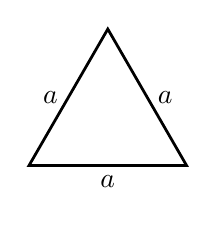
\begin{tikzpicture}[ampersand replacement=\&,line width=1pt]
            \draw (0,0) -- (60:2) node [midway,left] {$a$} -- + (-60:2) node [midway,right] {$a$} -- cycle node [midway,below] {$a$}; 
        \end{tikzpicture}
    \end{tcolorbox}
    \begin{tcolorbox}[adjusted title=Isósceles] 
        Tiene dos lados iguales \tcblower 
        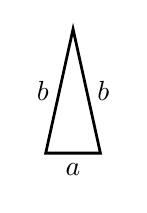
\begin{tikzpicture}[ampersand replacement=\&,line width=1pt,y=0.8cm]
            \draw (0,0) -- (80:2) node [midway,left] {$b$} -- + (-80:2) node [midway,right] {$b$} -- cycle node [midway,below] {$a$}; 
        \end{tikzpicture}
    \end{tcolorbox}
    \begin{tcolorbox}[adjusted title=Escaleno] 
        Tiene tres lados desiguales \tcblower 
        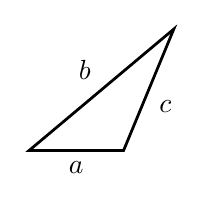
\begin{tikzpicture}[ampersand replacement=\&,line width=1pt,scale=0.6]
            \draw (2,0) -- (0,0) node [midway,below] {$a$} -- (40:4) node [midway,above left] {$b$} -- cycle node [midway,below right] {$c$};
        \end{tikzpicture}
    \end{tcolorbox}
    \begin{tcolorbox}[adjusted title=Ractángulo] 
        Tiene un ángulo recto \mbox{$(=90^{\circ})$} \tcblower 
        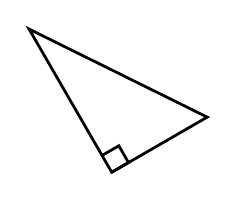
\begin{tikzpicture}[ampersand replacement=\&,line width=1pt,rotate=30,scale=0.7]
            \draw (0,3) -- (0,0) -- (2,0) -- cycle;
            \draw (0,0) -- ([turn]90:10pt) --  ([turn]90:10pt) --  ([turn]90:10pt);
        \end{tikzpicture}
    \end{tcolorbox}
    \begin{tcolorbox}[adjusted title=Acutángulo] 
        Tiene tres ángulos agudos $(<90^{\circ})$ \tcblower 
        \begin{tikzpicture}[ampersand replacement=\&,line width=1pt,scale=0.7]
            \draw  (0,0) coordinate (A) -- (70:3) coordinate (B) -- ([turn]-110:2) coordinate (C) -- cycle;
            \draw pic ["",draw,angle radius=15pt] {angle = A--B--C};
            \draw pic ["",draw,angle radius=15pt] {angle = C--A--B};
            \draw pic ["",draw,angle radius=12pt] {angle = C--A--B};
            \draw pic ["",draw,angle radius=15pt] {angle = B--C--A};
            \draw pic ["",draw,angle radius=12pt] {angle = B--C--A};
            \draw pic ["",draw,angle radius=18pt] {angle = B--C--A};
        \end{tikzpicture}
    \end{tcolorbox}
    \begin{tcolorbox}[adjusted title=Obtusángulo] 
        Tiene un ángulo obtuso \mbox{$(>90^{\circ})$} \tcblower 
        \begin{tikzpicture}[ampersand replacement=\&,line width=1pt,scale=0.6,rotate=10]
            \draw  (0,0) coordinate (A) -- (0:3) coordinate (B) -- ([turn]60:3) coordinate (C) -- cycle;
            \draw pic ["",draw,angle radius=15pt] {angle = C--B--A};

        \end{tikzpicture}
    \end{tcolorbox}
\end{tcbraster}

\section*{Para resolver}

\begin{ejercicios}
    \task! $\overline{AF} \parallel \overline{BE}$ y $\overline{CG}$ con $\overline{DH}$ tranversales. Usando 
    que $\angle JOK = 85^{\circ}$, $\angle OJK^{\circ} = 35$ y $\angle OKE = 120^{\circ}$, determina la medida de los 
    ángulos faltantes.
    \begin{center}
    \vspace{5pt}
    \begin{tikzpicture}[ampersand replacement=\&,line width=1pt]
        \coordinate (A) at (0,0);
        \coordinate (B) at (9,0);
        \pgfmathsetmacro{\dist}{3}
        \draw[<->,name path=l2] (A) node [left] {$l_2$} -- (B);
        \draw[<->,name path=l1] ($(A)+(0,\dist)$) node [left] {$l_1$} -- ($(B)+(0,\dist)$);
        \coordinate[] (G) at ($(A)!0.3!(B)!1.2!35:(B)$);
        \coordinate[] (C) at ($(A)!0.3!(B)!0.9!35:(A)$);
        \draw[<->,name path=l3]  (C) node[below] {$l_3$} -- (G);
        \coordinate[] (H) at ($(A)!0.6!(B)!1.4!120:(B)$);
        \coordinate[] (G) at  ($(A)!0.6!(B)!0.35!120:(A)$);
        \draw[<->,name path=l4] (G) node[below] {$l_4$} -- (H);
        \draw[dotted] ($(A)!0.3!(B)$) circle (20pt);
        \draw[dotted] ($(A)!0.6!(B)$) circle (20pt);
        \draw[name intersections={of=l1 and l4,by=p14},dotted] (p14) circle (20pt);
        \draw[name intersections={of=l3 and l4,by=p34},dotted] (p34) circle (20pt);
        \draw[name intersections={of=l1 and l3,by=p13},dotted] (p13) circle (20pt);
        \node[below=4pt,xshift=-2pt] at (p34) {$85^{\circ}$};
        \node[xshift=-28pt,yshift=-9pt] at ($(A)!0.3!(B)$) {$35^{\circ}$};
    \end{tikzpicture}
    \end{center}
    \task 
    Considerando la información entregada en la figura, ¿Qué se puede decir con respecto a las rectas $l_1$ y $l_2$?.
    \begin{center}
        \begin{tikzpicture}[ampersand replacement=\&,line width=1pt,rotate=60]
            \draw (0,0) coordinate[label=left:$l_1$] (A) -- + (-40:2) coordinate (B) -- ([turn]50:2) % 
            coordinate (C) -- ([turn]-50:2) coordinate (D) -- ([turn]180:4) coordinate[label=left:$l_2$] (E);
            \draw pic ["$\theta$",draw,angle radius=20pt] {angle = C--B--A};
            \draw pic ["$\theta$",draw,angle radius=20pt] {angle = B--C--D};
        \end{tikzpicture}
    \end{center}
    \task $l_1 \parallel l_2$, ¿Cuánto vale $\angle ABC$ + $\angle DEF$?.
    \begin{center}
    \vspace{5pt}
    \begin{tikzpicture}[ampersand replacement=\&,line width=1pt]
        \draw node [right] {$l_1$} (0,0) coordinate[label=above:$A$] (A) -- (180:4) coordinate[label=above:$B$] (B) %
        -- ([turn]120:1.8) coordinate[label=right:$C$] (C) -- ([turn]-70:2) coordinate[label=below:$D$] (D) % 
        -- ([turn]130:4) coordinate[label=below:$E$] (E) node [right] {$l_2$};
        \draw pic ["$60^{\circ}$",draw,angle radius=30pt] {angle=C--B--A};
        \draw pic ["$50^{\circ}$",draw,angle radius=30pt,angle eccentricity=0.7] {angle=E--D--C};
    \end{tikzpicture}
    \end{center}
    \task! $l_1 \parallel l_2 \parallel l_3$. Determinar el valor de $\angle CDE$ y $\angle FCD$.
    \begin{center}
    \begin{tikzpicture}[ampersand replacement=\&,line width=1pt]
        \draw node [left] {$l_1$} (0:0) coordinate[label=A] (A) -- + (0:4) coordinate[label=B] (B) %
        -- ([turn]-125:3) coordinate[label=below:C] (C) -- ([turn]157:2) coordinate[label=D] (D) % 
        -- ([turn]-32:3) coordinate[label=E] (E) node [right] {$l_2$};
        \draw (C) -- + (0:4) coordinate[label=below:F] (F) node [right] {$l_3$};
        \draw pic ["$55^{\circ}$",draw,angle radius=30pt] {angle=A--B--C};
        \draw pic ["$23^{\circ}$",draw,angle radius=50pt, angle eccentricity=0.85] {angle=D--C--B};
    \end{tikzpicture}
    \end{center} 
    \task! En el cuadrilátero $ABCD$, $\overline{AB}$ y $\overline{BC}$ son perpendiculares. Encuentre la medida de todos los
    ángulos desconocidos.
    \begin{center}
    \vspace{5pt}
    \begin{tikzpicture}[ampersand replacement=\&,line width=1pt]
        \draw (0,0) coordinate[label=left:$A$] (A) -- + (-30:7) coordinate[label=below:$B$] (B) % 
            -- ([turn]90:5) coordinate[label=right:$C$] (C) -- ([turn]80:3.5) coordinate[label=above:$D$] (D) -- cycle;
        \draw[dotted,name path=l1] (A) -- (C);
        \draw[dotted,name path=l2] (B) -- (D);
        \draw[name intersections={of=l1 and l2,by=pO},dotted] (pO) circle (25pt);
        \draw pic ["",draw,angle radius=35pt,dotted] {angle = B--A--D};
        \draw pic ["",draw,angle radius=35pt,dotted] {angle = A--D--C};
        \draw pic ["",draw,angle radius=35pt,dotted] {angle = D--C--B};
        \draw pic ["",draw,angle radius=35pt,dotted] {angle = C--B--A};
        \node[below right,xshift=15pt,yshift=2pt] at (A) {$35^{\circ}$};
        \node[below left,yshift=-3pt] at (pO) {$85^{\circ}$};
        \node[below left,yshift=-3pt,xshift=-7pt] at (C) {$25^{\circ}$};
        \node[below left,yshift=-10pt] at (D) {$75^{\circ}$};
    
    \end{tikzpicture}
    \end{center}
    \task La suma de los ángulos internos de un triángulo es de $180^{\circ}$, ¿cuál es la 
    suma de los ángulos interiores de una estrella de 8 puntas?
    \begin{center}
        \vspace{5pt}
        \begin{tikzpicture}[ampersand replacement=\&, line width=1pt]
            \node [shape=star,star points=8, star point ratio=2, inner sep=7mm, draw] {};
        \end{tikzpicture}
        \end{center}
    \task Un carpintero está construyendo una escalera, si cada plantilla es paralela al 
    piso y el larguero forma un ángulo de $43^{\circ}$ con el piso, encuentra el 
    ángulo $ABC$.
    \begin{center} 
        \vspace{5pt}
        \includegraphics[width=0.9\linewidth]{escalera.png}
    \end{center}
\end{ejercicios}

\end{document}